\begin{definition} \textbf{Paralelepípedo rectangular .}  Al conjunto $P  \subseteq  \mathbb{R}^3$ dado por
\[
P = \left\{ (x, y, z) \in \mathbb{R}^3 \;\middle|\; a \leq x \leq b,\; c \leq y \leq d,\; e \leq z \leq f \right\}
\] 
se lo llama paralelepípedo rectangular . 
\end{definition}


\begin{definition} \textbf{Partici\'on regular.} 	Sea \( P  \subseteq  \mathbb{R}^3 \) un paralelepípedo.  Una partición regular de $B$ es un conjunto de pequeños paralelepípedos disjuntos (salvo tal vez por sus caras)  de igual volumen que  generan una subdivisi\'on de $P$.  Es decir, si $P = [a, b] \times [c, d] \times [e, f]$,  esto se logra dividiendo:

\begin{itemize}
    \item el intervalo \( [a, b] \) en \( l \) subintervalos \( [x_i, x_{i+1}] \)  con $0 \leq  i \leq l-1$ cada uno de ancho \( \Delta x \),
    \item el intervalo \( [c, d] \) en \( p \) subintervalos \( [y_j, y_{j+1}] \)  con $0 \leq  p \leq p-1$, cada uno de ancho \( \Delta y \),
    \item el intervalo \( [e, f] \) en \( m \) subintervalos \( [z_k, z_{k+1}] \)  con $0 \leq  k \leq m-1$, cada uno de ancho \( \Delta z \).
\end{itemize}
y tomando los sub paralelepípedos $P_{ijk}$ tales que
	\[
	P_{ijk} = [x_i, x_{i+1}] \times [y_j, y_{j+1}] \times [z_k, z_{k+1}]
	\]  El volumne de $ P_{ijk}$ la notaremos por $\Delta P_{ijk}$ 
\end{definition}


%\input{figs/conjunto_B.tex}


\begin{definition}
Dada una funci\'on $f:P\to\R$, donde $P\subset \Rn{3}$ es un paralelep\'ipedo rectangular, se define la \emph{suma de Reimann}  de $f$ sobre $P$ a
\[
    S_{l,p,m}=\sum_{i=0}^{l-1}\sum_{j=0}^{p-1}\sum_{k=0}^{m-1}f(c_{ijk})\Delta P_{ijk},
\]  
donde $\{ P_{ijk}\}_{( 1 \leq i \leq l, 1 \leq j \leq p, 1 \leq k \leq m  )}$ es una partici\'on regular de $P$ y  $c_{ijk}\in P_{ijk}  \: \forall \: 1 \leq i \leq l, 1 \leq j \leq p, 1 \leq k \leq m.$ 
\end{definition}

\begin{definition} 
Sea $f: P=[a,b]\times[c,d]\times[e,f] \to\R$ una funci\'on.    Diremos que $f$ es integrable sobre $P$ si existe y es finito el  l\'imite $\lim_{(l,p,m)\to(\infty,\infty,\infty)} S_{l,p,m}$, en tal caso  el valor de dicho l\'imite  se llama \emph{integral triple} de $f$ sobre $P$ y se nota 
    \[
          \iiint_P f\:dV  \: \mbox{ o } \:  \iiint_P f(x,y,z)\:dxdydz.
    \]
\end{definition}






\begin{obs}
Para la existencia del límite anterior, se requiere $f$ acotada en $U$ y continua, excepto, tal vez, en la unión finita de gráficas de funciones 
contínuas, es decir, superficies.
\end{obs}


Para extender esta noci\'on de integral a  conjuntos acotados m\'as generales que no sean  paralelepípedos , definimos lo siguiente. 

\begin{definition}\label{def:caja-que-contiene} Sea $W  \subseteq  \mathbb{R}^3$ , $f:W\to\R$ continua y  $P = [a, b] \times [c, d] \times [e, f]$ tal que $W  \subseteq  P$.  Se define la funci\'on $f^*$ tal que
\[
    f^*(x,y,z)=
    \begin{dcases*}
        f(x,y,z) & si $(x,y,z)\in W$ \\[.2cm]
        0        & si $(x,y,z)\notin P\smallsetminus W.$
    \end{dcases*}
\]
La inegral de  $f$ sobre $W$ se define por 
\[
    \iiint_W f\:dV=\iiint_P f^*\:dV.  
\]
\end{definition}

\begin{obs} 
   La \autoref{def:caja-que-contiene} es independiente de la selecci\'on de $P$.
\end{obs}

\begin{propertie}
    Sean $f,\;g$ dos funciones integrables en una regi\'on $W\subset\Rn{3}$, entonces:
    \begin{enumerate}
        \item[i.] $\alpha f+\beta g$ es integrable en $W$, $\forall\;\alpha,\;\beta\in\R$ y adem\'as
        \[
            \iiint_W \left(\alpha f+\beta g\right)dV=\alpha\iiint_W f\:dV+\beta\iiint_W g\:dV.
        \]
        \item[ii.] El producto $fg$ es integrable en $W$.
        \item[iii.] Si $g(x,y,z) \neq  0\;\forall(x,y,z)\in W$ entonces el cociente $f/g$ es integrable en $W$.
        \item[iv.] Si $f(x,y,z) \geq 0  \;\: \forall(x,y,z)\in W$ entonces  $\iiint_W f\:dV\geq0$.
        \item[v.]Si $f(x,y,z) \leq g(x,y,z) \;\: \forall(x,y,z)\in W$ entonces $\iiint_W f\:dV\leq\iiint_W g\:dV.$
        \item[vi.]Si $|f|$ es integrable en $W$, entonces 
        \[
            \left|\iiint_W f\:dV\right|\leq\iiint_W|f|\:dV.  
        \]    
        \item[vii.] Si $W=W_1\cup W_2$  con $W_1\cap W_2 = \varnothing$  (salvo tal vez en conjuntos de medida nula): 
        
        $f$ es integrable en $W$ $\iff$ $f$ es integrable en $W_1$ y $W_2$.
        
         En este caso 
        \[
            \iiint_W f\:dV=\iiint_{W_1} f\:dV+\iiint_{W_2}f\:dV.    
        \]
    \end{enumerate}
\end{propertie}

\begin{definition} Sea $W\subset\Rn{3}$,  se define el volumen de $W$,  y se nota $\text{Vol}(W)$,  a  
    
    \[
        \text{Vol}(W)=\iiint_W 1 \:dV.
    \]
\end{definition}


\begin{definition}
    \textbf{Conjunto elemental en }$\Rn{3}$. Sean $D_i\in \Rn{2}$ con $1 \leq i \leq 3$  cunjuntos elementales y sean $\eta_{1i}$ y $\eta_{2i}$  con $1 \leq i \leq 3$ funciones continuas sobre $D_i$ .  Un conjunto $W\subseteq\Rn{3}$ se llama elemetal si puede ser descripto de alguna de las siguientes maneras. 
    \begin{enumerate}
    \item Exiten $D_1 \subset  \mathbb{R}^2 $ un conjunto elemental y funciones  $\eta_{11},\; \eta_{21}: D_1\to\R$  continuas  tales que $$\eta_{11}(x, y) <  \eta_{21}(x, y)  \: \forall (x,y) \in  (D_1)^{\circ}$$ y $$ W = \left\{ (x, y, z) \in \mathbb{R}^3 \;\middle|\;  (x,y) \in D_1 \: \land  \: \eta_{11}(x, y) \leq z \leq \eta_{21}(x, y)  \: \forall (x,y) \in D_1 \right\}.$$
	
	
	\item  Exiten $D_2 \subset  \mathbb{R}^2 $ un conjunto elemental y funciones  $\eta_{12},\; \eta_{22}: D_2\to\R$  continuas  tales que $$\eta_{12}(x, z) <  \eta_{22}(x, z)  \: \forall (x,z) \in  (D_2)^{\circ}$$ y $$W = \left\{ (x, y, z) \in \mathbb{R}^3 \;\middle|\;  (x,z) \in D_2   \: \land  \:  \eta_{12}(x, z) \leq y \leq \eta_{22}(x, z) \: \forall (x,z) \in D_2 \right\}$$
	
	\item  Exiten $D_3 \subset  \mathbb{R}^2 $  un conjunto elemental y funciones  $\eta_{13},\; \eta_{23}: D_3\to\R$  continuas  tales que $$\eta_{13}(y, z) <  \eta_{23}(y, z)  \: \forall (y,z) \in  (D_3)^{\circ}$$ y $$W = \left\{ (x, y, z) \in \mathbb{R}^3 \;\middle|\; (y,z) \in D_3   \: \land  \:  \eta_{13}(y, z) \leq x \leq \eta_{23}(y, z) \: \forall (y,z) \in D_3  \right\}$$
\end{enumerate}
\end{definition}

%\begin{center}    
   % 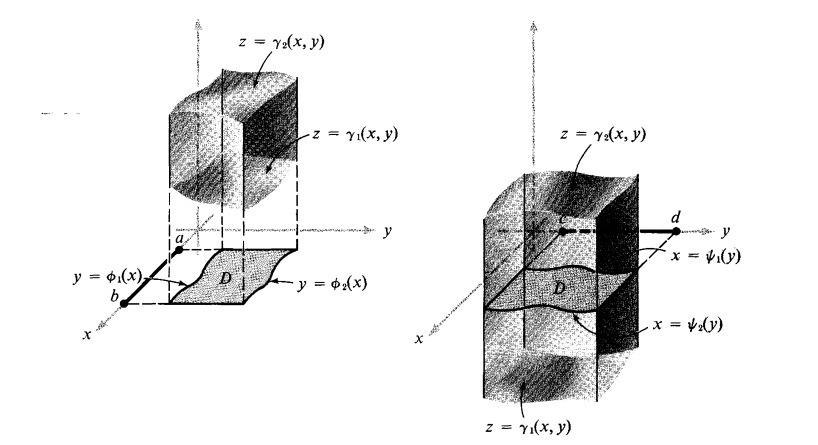
\includegraphics[width=0.8\linewidth]{figs/conj_elem_r3.jpg}
%\end{center}

\begin{theorem} \textbf{Teorema del valor medio.}   Sea $f:W\subseteq\Rn{3}\to\Rn{3}$ continua.  Entonces existe $(x_0,y_0,z_0) \in W$ tal que 
    \[
        \iiint_W f\:dV=f(x_0,y_0,z_0)\text{Vol}(W).
    \]
\end{theorem}





\begin{theorem}
    \textbf{Teorema del cambio de variables para integrales triples.}  Sean $W \subseteq\Rn{3}$ un conjunto acotado y  $f:W \to\R$ un campo integrable sobre $W$ y sea $\mathbf{T}:W^*\subseteq\Rn{3}\to W\subseteq\Rn{3}$ continua en $W^*$, de clase $\mathcal{C}^1(\interior{(W^*)})$,  inyectiva en $\interior{(W^*)}$ y tal que $\mathbf{T}(W^*)=W$.  Entonces
    \[
        \iiint_W f\:dV=\iiint_{W^*}(f\circ\mathbf{T})J_\mathbf{T}\:dV.
    \]
\end{theorem}







